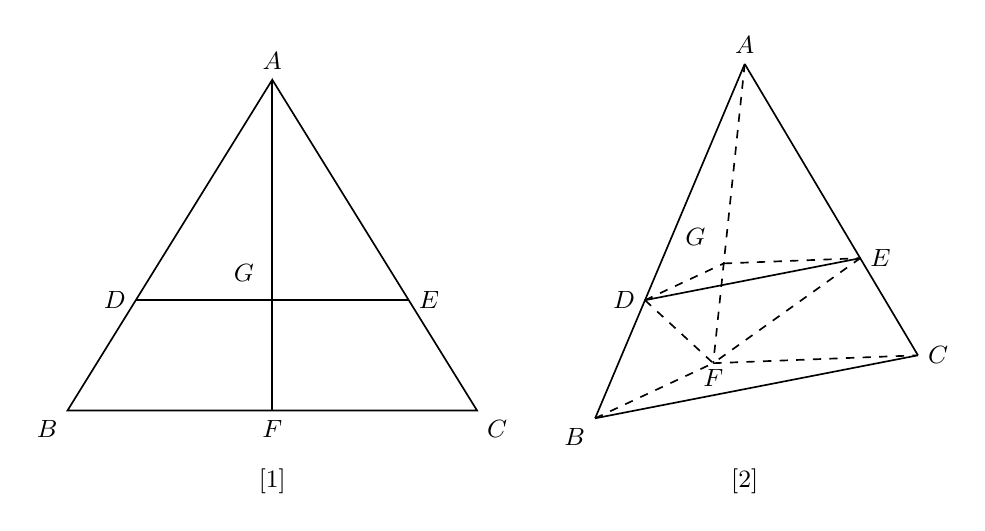
\begin{tikzpicture}[line width=.6pt, font=\small, >=stealth]
% ---- left panel plane triangle (schematic, exact incidences) ----
\coordinate (A) at (0,4.2);
\coordinate (B) at (-2.6,0);
\coordinate (C) at (2.6,0);
\coordinate (F) at (0,0);
\coordinate (D) at (-1.7333333333,1.4000000000);
\coordinate (E) at (1.7333333333,1.4000000000);
\coordinate (G) at (0.0000000000,1.4000000000);
\draw (A)--(B)--(C)--cycle;
\draw (A)--(F);
\draw (D)--(E);
\node[above] at (A) {$A$};
\node[left] at (D) {$D$};
\node[above left=3pt] at (G) {$G$};
\node[right] at (E) {$E$};
\node[below left] at (B) {$B$};
\node[below] at (F) {$F$};
\node[below right] at (C) {$C$};
\node at (0,-0.9) {\bitmapinsertcaption[1]};
% ---- right panel tetrahedron A-BCF ----
\coordinate (Ar) at (6,4.4);
\coordinate (Br) at (4.1,-0.1);
\coordinate (Cr) at (8.2,0.7);
\coordinate (Fr) at (5.6,0.6);
\coordinate (Dr) at (4.7333333333,1.4000000000);
\coordinate (Er) at (7.4666666667,1.9333333333);
\coordinate (Gr) at (5.7333333333,1.8666666667);
% solid outer
\draw (Ar)--(Br);
\draw (Ar)--(Cr);
\draw (Br)--(Cr);
% dashed hidden / interior
\draw[dashed] (Ar)--(Fr);
\draw[dashed] (Br)--(Fr);
\draw[dashed] (Fr)--(Cr);
\draw (Dr)--(Er);
\draw[dashed] (Dr)--(Gr);
\draw[dashed] (Gr)--(Er);
\node[above] at (Ar) {$A$};
\node[below left] at (Br) {$B$};
\node[right] at (Cr) {$C$};
\node[below=2pt,inner sep=0pt,font=\small] at (Fr) {$F$};
\node[left] at (Dr) {$D$};
\node[right] at (Er) {$E$};
\node[above left=3pt] at (Gr) {$G$};
\node at (6,-0.9) {\bitmapinsertcaption[2]};
\draw[dashed] (Dr)--(Fr)--(Er);
\end{tikzpicture}
